%%%%%%%%%%%%%%%%%%%%%%%%%%%%%%%%%%%%%%%%%
% Research Report Assignment Title Page 
% LaTeX Template
% Version 1.0 (06/03/16)
%
% This template has been downloaded from:
% http://www.LaTeXTemplates.com
%
% Original author: Francisco Maria Calisto
% WikiBooks (http://en.wikibooks.org/wiki/LaTeX/Title_Creation)
%
% License:
% CC BY-NC-SA 3.0 (http://creativecommons.org/licenses/by-nc-sa/3.0/)
% 
% Instructions for using this template:
% This title page is capable of being compiled as is. This is not useful for 
% including it in another document. To do this, you have two options: 
%
% 1) Copy/paste everything between \begin{document} and \end{document} 
% starting at \begin{titlepage} and paste this into another LaTeX file where you 
% want your title page.
% OR
% 2) Remove everything outside the \begin{titlepage} and \end{titlepage} and 
% move this file to the same directory as the LaTeX file you wish to add it to. 
% Then add \input{./title_page_1.tex} to your LaTeX file where you want your
% title page.
%
%%%%%%%%%%%%%%%%%%%%%%%%%%%%%%%%%%%%%%%%%
%\title{Title page with logo}
%------------------------------------------------------------------------------
%	PACKAGES AND OTHER DOCUMENT CONFIGURATIONS
%------------------------------------------------------------------------------

\documentclass[12pt]{article}
\usepackage[english]{babel}
\usepackage[utf8x]{inputenc}
\usepackage[T1]{fontenc}
\usepackage{amsmath}
\usepackage{graphicx}
\usepackage[colorinlistoftodos]{todonotes}
\usepackage{subcaption}
\usepackage{biblatex}
\usepackage{fontspec}

\addbibresource{bib.bib}

\begin{document}

\begin{titlepage}

\newcommand{\HRule}{\rule{\linewidth}{0.5mm}} % Defines a new command for the horizontal lines, change thickness here

\center % Center everything on the page
 
%------------------------------------------------------------------------------
%	HEADING SECTIONS
%------------------------------------------------------------------------------

% Name of your university/college
\textsc{\LARGE Instituto Superior T\'{e}cnico}\\[1.5cm]
% Major heading such as course name
\textsc{\Large ISR}\\[0.5cm]
% First Minor heading such as course title
\textsc{\large Report}\\[0.25cm]
% Second Minor heading such as course title
\textsc{\small Conceptual Model Milestone}\\[0.25cm]

%------------------------------------------------------------------------------
%	TITLE SECTION
%------------------------------------------------------------------------------

\HRule \\[0.5cm]
{ \large \bfseries  Participatory Task Modelling Prototype Meeting}\\[0.25cm] % Title of your document
\HRule \\[0.5cm]
 
%------------------------------------------------------------------------------
%	AUTHOR SECTION
%------------------------------------------------------------------------------

\begin{minipage}{0.4\textwidth}
\begin{flushleft} \large
\emph{Author:}\\
Francisco Maria \textsc{Calisto} % Your name
\end{flushleft}
\end{minipage}
~
\begin{minipage}{0.4\textwidth}
\begin{flushright} \large
\emph{Coordinator:} \\
Jacinto \textsc{Nascimento} % Coordinator's Name
\end{flushright}
~
\begin{flushright} \large
\emph{Co-Coordinator:} \\
Daniel \textsc{Gon\c{c}alves} % Co-Coordinator's Name
\end{flushright}
\end{minipage}\\[2cm]

% If you don't want a supervisor, uncomment the two lines below and remove the section above
%\Large \emph{Author:}\\
%John \textsc{Smith}\\[3cm] % Your name

%-----------------------------------------------------------------------------
%	DATE SECTION
%-----------------------------------------------------------------------------

{\large 11/08/2016}\\[1cm] % Date, change the \today to a set date if you want to be precise

%-----------------------------------------------------------------------------
%	LOGO SECTION
%-----------------------------------------------------------------------------

% 
\includegraphics{ist-logo.png}\\[0.5cm] % Include a department/university logo - this will require the graphicx package

% 
\includegraphics{isr-logo.png}\\[0.5cm] % Include a department/university logo - this will require the graphicx package

\begin{figure}
\centering
\begin{subfigure}{.5\textwidth}
  \centering
  
\includegraphics[width=.5\linewidth]{isr-logo.png}
\end{subfigure}%
\begin{subfigure}{.5\textwidth}
  \centering
  
\includegraphics[width=.5\linewidth]{inesc-id-logo.png}
\end{subfigure}
\begin{subfigure}{.5\textwidth}
  \centering
  
\includegraphics[width=.25\linewidth]{ist-logo.png}
\end{subfigure}
\end{figure}
 
%-----------------------------------------------------------------------------

\vfill % Fill the rest of the page with whitespace

\end{titlepage}

\section{Abstract}

Clinical researchers aim to maintain multi-modal, speciality-specific images with associated high-quality data for purposes of diagnosing breast cancer.

As hospital information systems are not designed to record breast cancer diagnosis, physicians need to gather appropriate sets of visualisation to facilitate the clinical activity. To include the physicians in the design and development of a new health information system, we adopt the Participatory Task Modelling (PTM) \cite{o2004participatory, keungparticipatory} approach for user requirement gathering and development.

This report describes our experience on the prototyping developments and aims to report the demonstration of some of the first prototypes developed in Balsamiq \cite{Balsamiq} and beyond also understand how is made all breast activity diagnosis approaching within the main care research domain, and discusses the challenges encountered.

\clearpage

\section{Introduction}

Hospital information systems in Portugal are mainly used as clinical diagnosis activities and record patients. For clinical and research purposes, physicians have routinely been using separate systems for this diagnosis. Thus, are using the many systems as tools of multimodality of imaging but not as integrated in one tool. The visualisation becomes poor and entropic, with the need of consolidation.

To encourage our physicians to participate with made a set of prototypes that will bring our questions into what will be a best answer to a breast cancer multi-modality of image user interface, supporting our clinical research, in particular physicians cohort identification and analysis phases for clinical studies and trials.

\clearpage

\section{Task Modelling}

The report focuses on one medical speciality, Radiologist Doctors, for the development of breast cancer multi-modality of image user interface research. To capture the user requirements and the domain-specific context, we are actively involving the users in the design of the system through hospital meetings.

Task analysis comprises a wide range of development activities and research, including modelling of the task domain, data collection and data analysis (e.g.: surveys). Task analysis has mainly involved users at the data gathering stage, while the analysts are mainly involved in the data analysis and the modelling of users’ tasks and surveys, since participatory design, in comparison, encourages the involvement of users with developers in the systems development activities \cite{muller1993taxonomy}.

The quality of data collated is a product of tools and techniques adopted. Requirement specifications templates, wireframing tools (e.g. Balsamiq Mockups \cite{balsamiqMockups}) and frequent iterative knowledge elicitation consultations with stakeholders play a key role our implementation of the PTM approach. Furthermore, we have used existing systems, where applicable, as the basis for requirements gathering. The cooperation between researchers and physician users has been an important part of our work to enable the correct interpretation of tasks and terminology, as well as to understand to a certain extent the workplace culture and politics \cite{williams1993translation}.

Our cooperation has work experience in both the health domain and user interface development, and supports in the identification of possible miscommunication between physicians and researchers. The use of mock-ups helps to simulate and validate the user interface and workflow, as well as improve on the limitations of traditional specification documents by engaging the users in a familiar environment.

\clearpage

\section{Low-Fidelity Prototypes Validation}

Base on the understanding of MIMBCD-UI system and the requirements from the user, the interface development can be triggered. The ultimate goal for this report and milestone (Conceptual Model Milestone) is to implement the design into MIMBCD-UI, so the interface development is developed as interface prototypes. Balsamiq Mockups \cite{Balsamiq} is a rapid wire framing tool which can build a rapid prototype in the software engineer, as said before. It can be used to draw an interface sketch for user interaction.

Once physicians like the design, it can be treated as the High Fidelity Prototypes. Interface design is the most critical part in this report. It should follow the UI design n rules and meets user’s need at the same time.

The final design of this milestone should meet following requirements:

- The UI should provide a support for user to understand the multi-modality of imaging interaction. So physicians can better diagnose breast cancer.

- The UI should help the user understanding where are the breast masses and calcifications.

- The UI should help young inexperienced radiologists to quickly familiar with
user interface.

- The UI must allow the physician to visualize the three modalities (Mammography, Ultrasound and MRI) in different screens levels and sizes measuring and diagnosis breasts.

As usual in this phases, the next prototypes are just drafts and are far from being finished and delivery into a master thesis. Some versions of prototypes can be seen in the MIMBCD-UI GitHub Repository at Lo-Fi Prototypes source \cite{mimbcdUILoFiPrototypes}.

\clearpage

A first statement physicians made was the idea of compare the last two images acquisitions on a main screen, but it is logic that this can't be the first screen to apear. However the preferences were made, we must have a clear option screen as first to choose the patients name and days (Figure 2).

% Commands to include a figure:
\begin{figure}[!hbt]
\centering
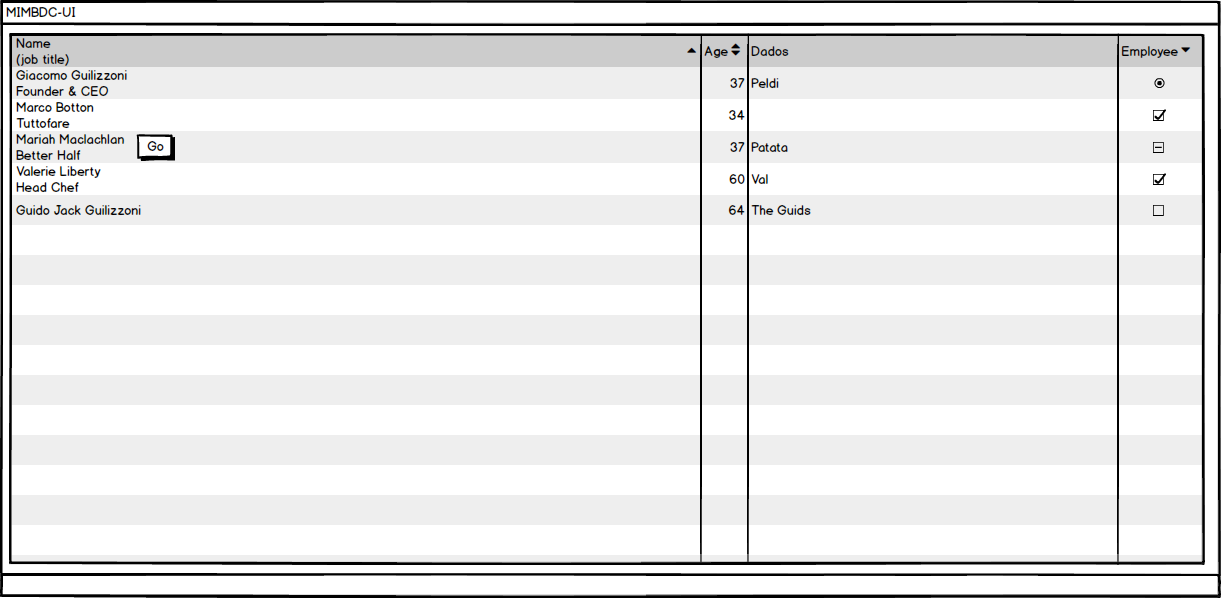
\includegraphics[width=1.00\textwidth]{tabela_pessoas.png}
\caption{\label{PT}Table of People.
}
\end{figure}

\clearpage

The second screen will have four of the multi-modality of imaging as we can see on Figure 3, and we will consider this the main screen, since the patient were already chosen.

% Commands to include a figure:
\begin{figure}[!hbt]
\centering
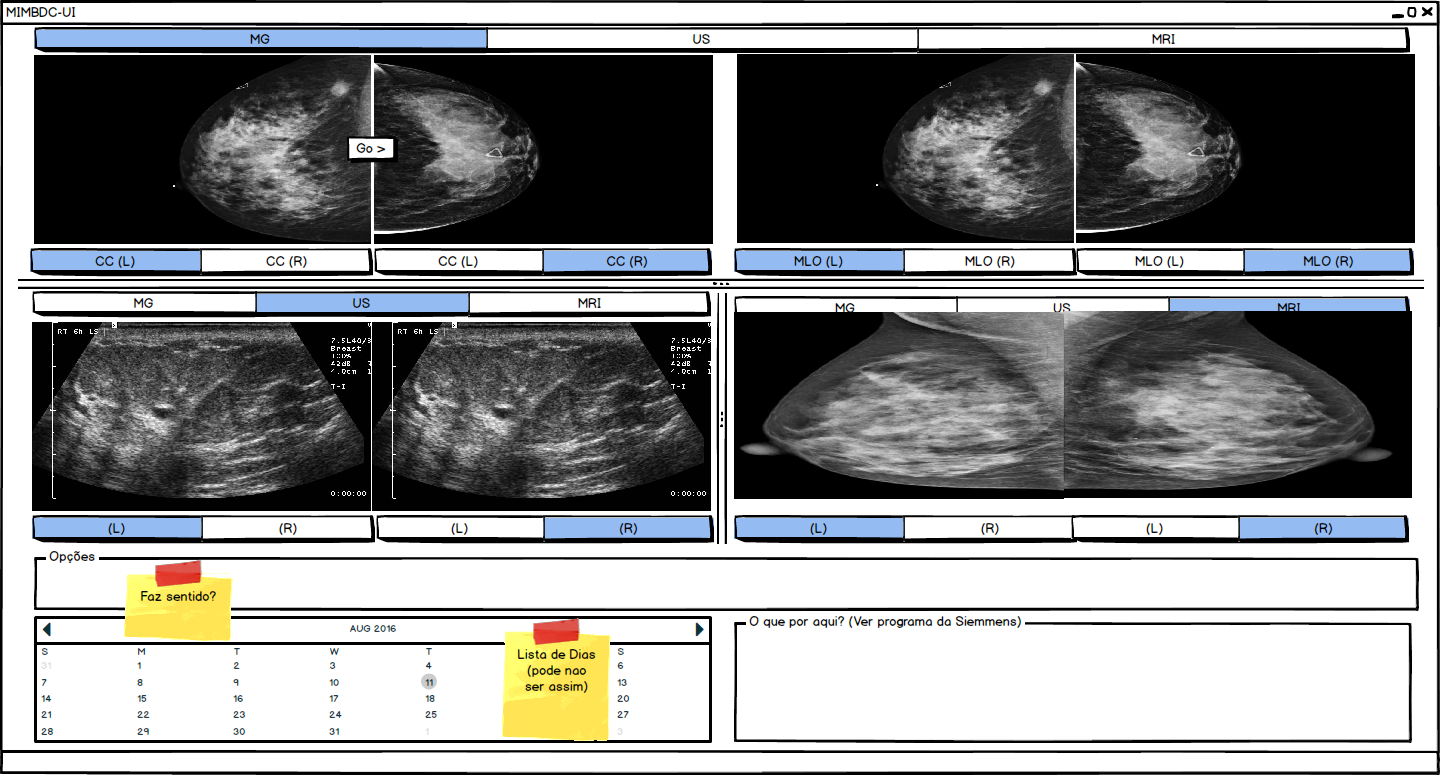
\includegraphics[width=1.00\textwidth]{multimodalidade.png}
\caption{\label{MMI}Multi-Modality of Imaging.
}
\end{figure}

\clearpage

From the necessity of having the set of CC and MLO screen views we implement a prototype with most of the screen directing to this option as we could seen on Figure 3 above. On the other hand, it was not enough to show just this screen options and it is fundamental to have a set of screens with the CC and MLO compared each other by the last two date image acquisitions.

% Commands to include a figure:
\begin{figure}[!hbt]
\centering
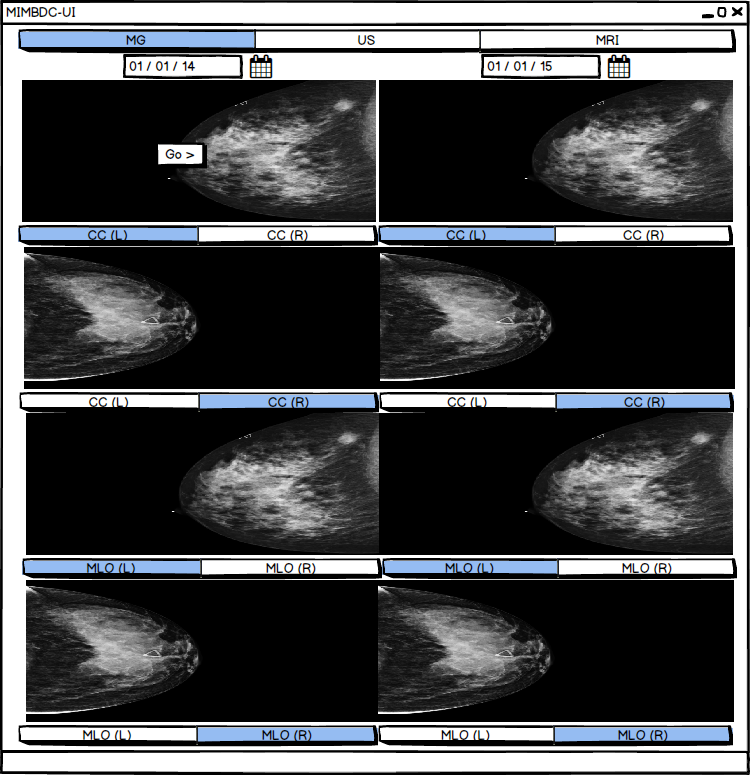
\includegraphics[width=1.00\textwidth]{MG_(Group).png}
\caption{\label{fig:PTM}Mammography Example (Group).
}
\end{figure}

\clearpage

\section{Discussion}

Using a PTM \cite{keungparticipatory} approach to gather user interface requirements and to model prototypes for analysis and design activities. Actively involving the physicians from an early stage and the support of a cooperation have led the researchers to be more aware of the medical research context.

% Commands to include a figure:
\begin{figure}[!hbt]
\centering
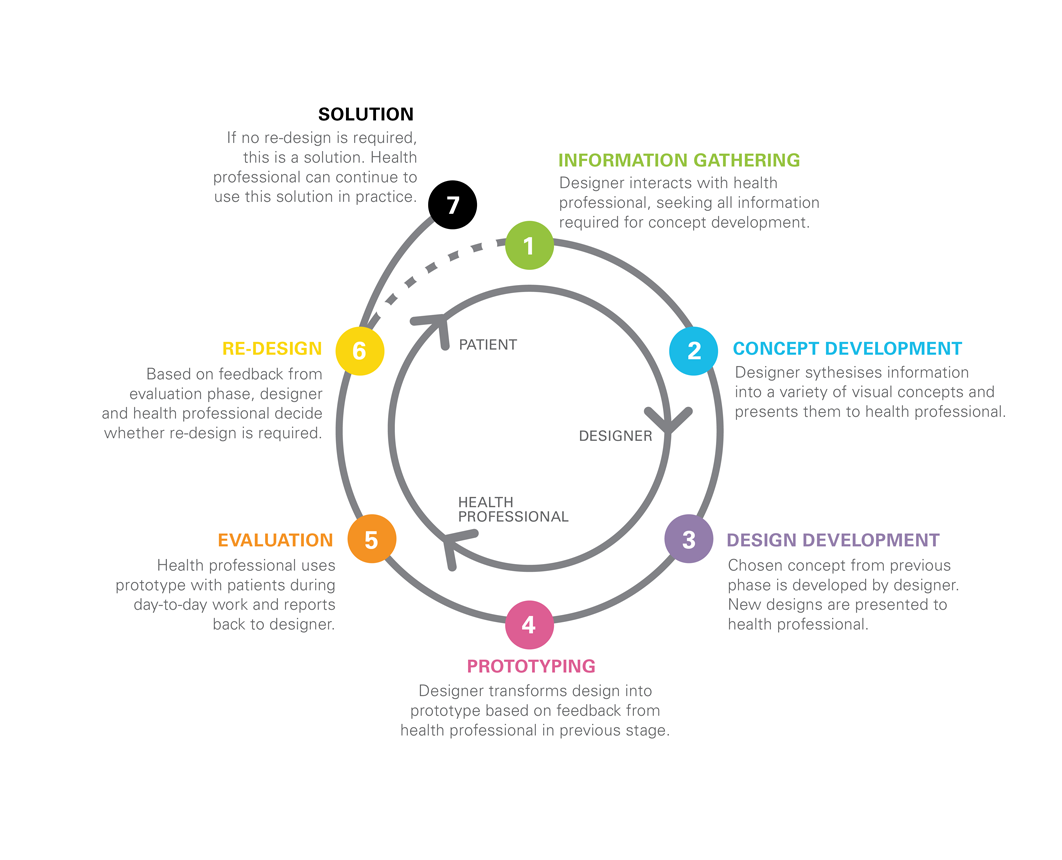
\includegraphics[width=1.00\textwidth]{ptm.png}
\caption{\label{fig:PTM}Participatory Task Modelling (PTM).
}
\end{figure}

For instance, as this report is dealing with research registries, many of the user requirements in terms of data to be collected are themselves research questions for the users. As a consequence, the occurrence of physicians changing their requirements is highlighted even further in this domain.

\clearpage

Despite the issues involved in the stakeholder consultations (e.g. organising meetings, participatory equality issues and surveys), their involvement is crucial in accurately representing user requirements. This report also aim to use the PTM approach in subsequent phases of the user interface life cycle where appropriate.

\section{Conclusions}

In this report, a user interface which is mainly facing to the diagnosis of breast cancer for the multi-modality of imaging was prototyped. MIMBCD-UI already has similar CAD \cite{wikiCAD} user interfaces, which is primarily for the researchers a base comparison. The work from this report has the potential to make physicians can also benefit from it. The UI design will base on the understanding of the current CAD \cite{wikiCAD} user interfaces and the MIMBCD-UI case library.

The depth observation and horizontal comparison of the MIMBCD-UI data, we found out that the difference in postoperative pain among different physicians group does exist. The CAD \cite{wikiCAD} theme is being an efficient way in dealing with this kind of data base. The interface is designed for the current CAD \cite{wikiCAD}, PACS \cite{wikiPACS} and DICOM \cite{wikiDICOM} example systems. It will be developed as the HTML, CSS and JavaScript prototype. So it can be implemented into the current system in the future.

\clearpage

\section{Acknowledgements}

This report will help our research project in cooperation between ISR \cite{isr} and INESC-ID \cite{inescid} both are associate laboratories institutes of Instituto Superior T\'{e}cnico \cite{ist}, Universidade de Lisboa \cite{ul}. Throughout this challenging journey we had the untiring and patient support from our family and friends.

We would like to give a special thanks to Dr. Cristina Ribeiro da Fonseca and Dr. Clara Aleluia who have cooperated with us tirelessly thus making a major contribution to the national research and development of innovation in Portugal medicine.

We also want to thanks Bruno Cardoso, Bruno Oliveira, Tom\'{a}s Pinho, L\'{i}dia Freitas, Bruno Dias, Jo\~{a}o Miranda, Prof. Dr. Jacinto Nascimento, Prof. Dr. Daniel Gon\c{c}alves, Ana Beatriz Alves, Francisco Silveira, Joana Teixeira, Daniel Da Costa, Filipe Fernandes, In\^{e}s Fran\c{c}a Martins, Lu\'{i}s Ribeiro Gomes and Ricardo Cruz for helping, support and review our work.

\clearpage

\printbibliography

\end{document}
